\section{Temperature Acquisition Channel}

	\subsection{Thermocouple Type and Signal}	
			
	 For this project it was defined that thermocouples of type K (formed by the junction of two metal leagues: Alumel and Cromel) would be used in this project. This is because this specific type of thermocouple has a wide range of operation (-200$^{\circ}$C - 1200 $^\circ}$C), so according to the requirements they are never too close from the boundary values, a thermocouple of type T or even a type J would not be suitable. Other appealing factor is that this type of thermocouple is quite common so getting eventual replacements would be easier, in comparisson with type E thermocouples.

	\subsection{Thermocouple Signal Conditioning}
	
	As mentioned in sub-section \ref{ssec:thermocouple}, besides amplification and linearization, the thermocouple signal also needs it's cold junction temperature difference compensation. There is an integrated solution from \textit{Analog Device} called AD8495, this IC functional diagram is displayed on Figure \ref{fig:ad8495-functional-block}.
	
		\begin{figure}[htbp]
			\centering
				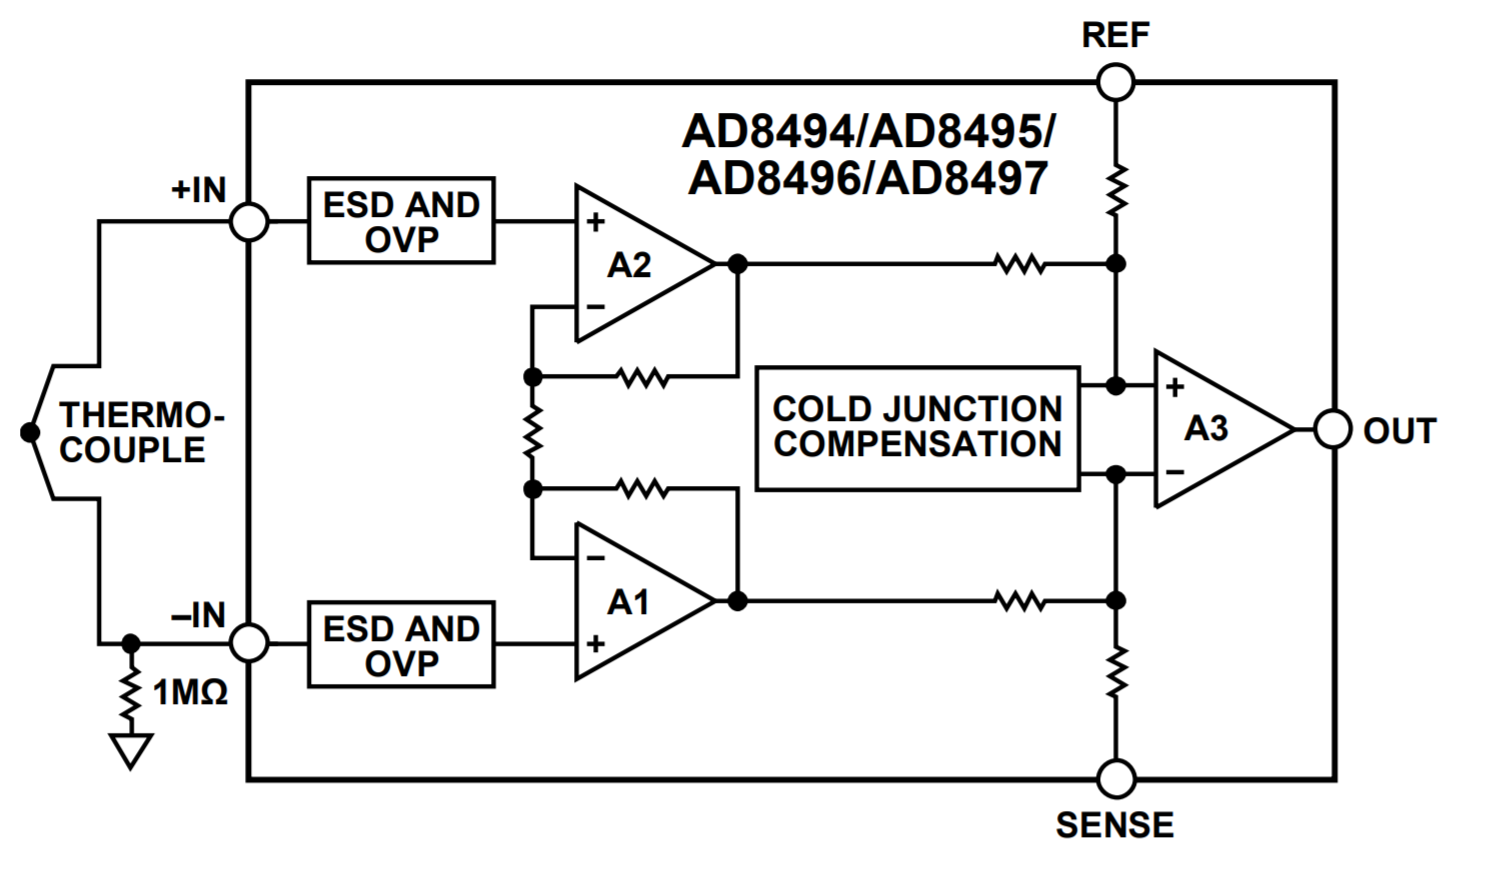
\includegraphics[scale=0.65]{figuras/fig-ad8495-functional-block}
			\caption{AD8495 Functional Block Diagram \cite{ad8495-functional-block}}
			\label{fig:ad8495-functional-block}
		\end{figure}
		
	This IC produces a linearized output with a fixed gain of $5mv\/^\circ}$C, it is a quite practical solution as it can be powered with single-supply voltage source and it's output saturates to the power supply voltage if the thermocouple is disconnected \cite{ad8495-datasheet}.
	
	\subsection{Input Protection and Filtering}\label{ssec:ad8495InputProtectionAndFiltering}
	
	Although this IC already has overvoltage and ESD protection, thermocouples tips can pick a load of unwanted noise and transients. Hence, additional protection and external filtering is also recommended by \cite{two-ways-thermocouple}. First thing to do is to add current-limint series resistors, the drawback is doing that is that resistors in the circuit net increases the overall noise. This type of noise is called Johnson-Nyquist Thermal Noise or more commonly just by Johnson Noise, thermal agitation of electrons in a resistor gives rise to random fluctuations in the voltage across its terminals \cite{romero1998johnson}. Moreover, it can be calculated using the following Equation \ref{eqn:johnson-noise} where K is the Boltzamann's constant $1.38 \cdot 10^{-23}$, R is the resistance in ohms $(\Omega)$ and T the temperature in kelvin (~300K at room temperature) \cite{sensors2000}.
	
		\begin{equation}\label{eqn:johnson-noise}
			Noise (nv\/\sqrt{Hz}) = \sqrt{4 \cdot K \cdot R \cdot T \cdot 10^{9}}
		\end{equation}
		
	Because the protection circuit includes two equal resistors, whose noise is uncorrelated, that is, the two noise sources are independent of each other—the above result must be multiplied by the square root of 2 (the root sum square of the two noise voltages) and it is considered as a general rule design to tolerate additional Johnson Noise from 10 to 30$\%$ to the amplifier IC \cite{sensors2000}. \cite{two-ways-thermocouple} suggests using current-limiting resistors of 10$k\Omega$, according to the AD8495 datasheet \cite{ad8495-datasheet}, the choosen amplifier (AD8495) has a voltage noise density of 32nV$\/ \sqrt{Hz}$. Combining this resistors noise with the amplifier noise will produce a overall noise of 36.85nV$\/\sqrt{Hz}$, which is just 13$\%$ above the amplifier's own noise. Additional protection can be achieved using external protection diodes as on Figure \ref{fig:externalProtectionDiodes}.
	
		\begin{figure}[htbp]
			\centering
				\includegraphics[scale=0.65]{figuras/fig-externalProtectionDiodes}
			\caption{External Protection Diodes \cite{externalProtectionDiodes}}
			\label{fig:externalProtectionDiodes}
		\end{figure}
		
	A Transient Voltage Suppression Diode (TVS) can be used to protect the inputs from differential input overvoltage, considering a bidirectional TVS with a 5V breakdown voltage, the device will theoretically limit the differential voltage between 5V and -5V, the AD8495 has overvoltage protection from -25V to 20V when powered with 5V, so this will successfully protect the amplifier inputs. It is also interesting to clamp each input to the supply rails using, this is best done using Schottky diodes, this type of diode operates the same way as standard diodes but have faster response and lower forward voltage. Schottky diodes have a foward voltage of approximately 200mV, if the supply rails are of 5V and 0V, a pair of diodes connected in the same way of Figure \ref{fig:externalProtectionDiodes}, the inputs will be clamped on -200mV and 5200mV, protecting the input.
	\par
	With the overloads protection done, another important feature to do is to filter unwanted signals in the inputs to avoid them to be amplified later

	\subsection{Thermocouple Sensor Detection}
		 

